\documentclass[aps,prl,reprint,superscriptaddress]{revtex4-1}
%\documentclass[aps,prl,reprint,superscriptaddress,hidelinks,nobalancelastpage,longbibliography]{revtex4-1}% for checking your page length
%\documentclass[aip,apl,preprint,graphicx]{revtex4-1} % for review purposes
\usepackage{amsmath,braket}
\usepackage{graphicx}
\usepackage{color}
\usepackage{hyperref} 
%\usepackage{float}
\usepackage[separate-uncertainty=true,multi-part-units=single]{siunitx}

%\draft % marks overfull lines with a black rule on the right

% APL Guidelines: 3500 words = 4 pages in "reprint"


\let\Re\relax
\DeclareMathOperator{\Re}{Re}
\let\Im\relax
\DeclareMathOperator{\Im}{Im}
\DeclareMathOperator{\Tr}{Tr}
%\textit{\textbf{}}
\definecolor{darkgreen}{rgb}{0.0,0.4,0.0}
%\sisetup{color = darkgreen}
%\sisetup{parse-numbers = false}
\DeclareSIUnit{\mu}{\micro\meter}
\DeclareSIUnit{\unit}{\relax}


\newcommand{\beginsupplement}{%
        \setcounter{table}{0}
        \renewcommand{\thetable}{S\arabic{table}}%
        \setcounter{figure}{0}
        \renewcommand{\thefigure}{S\arabic{figure}}%
     }



\begin{document}

% Use the \preprint command to place your local institutional report number 
% on the title page in preprint mode.
% Multiple \preprint commands are allowed.
%\preprint{}

\title{Demonstrating the decoupling regime of the electron-phonon interaction in a quantum dot using chirped optical excitation: Supplementary Information}

% repeat the \author .. \affiliation etc. as needed
% \email, \thanks, \homepage, \altaffiliation all apply to the current author.
% Explanatory text should go in the []'s, 
% actual e-mail address or url should go in the {}'s for \email and \homepage.
% Please use the appropriate macro for the type of information

% \affiliation command applies to all authors since the last \affiliation command. 
% The \affiliation command should follow the other information.


\author{Timo Kaldewey}
\affiliation{Department of Physics, University of Basel, Klingelbergstrasse 82, CH-4056 Basel, Switzerland}

\author{Sebastian L\"{u}ker}
\affiliation{Institut f\"{u}r Festk\"{o}rpertheorie, Universit\"{a}t M\"{u}nster, Wilhelm-Klemm-Strasse 10, D-48149 M\"{u}nster, Germany}

\author{Andreas V.\ Kuhlmann}
\affiliation{Department of Physics, University of Basel, Klingelbergstrasse 82, CH-4056 Basel, Switzerland}
\affiliation{IBM Research-Zurich, S\"{a}umerstrasse 4, CH-8803 R\"{u}schlikon, Switzerland}

\author{Sascha R.\ Valentin}
\affiliation{Lehrstuhl f\"{u}r Angewandte Festk\"{o}rperphysik, Ruhr-Universit\"{a}t Bochum, D-44780 Bochum, Germany}

\author{Jean-Michel Chauveau}
\affiliation{ Universit\'{e} C\^{o}te d'Azur, CNRS, CRHEA, France}

\author{Arne Ludwig}
\affiliation{Lehrstuhl f\"{u}r Angewandte Festk\"{o}rperphysik, Ruhr-Universit\"{a}t Bochum, D-44780 Bochum, Germany}

\author{Andreas D.\ Wieck}
\affiliation{Lehrstuhl f\"{u}r Angewandte Festk\"{o}rperphysik, Ruhr-Universit\"{a}t Bochum, D-44780 Bochum, Germany}

\author{Doris E. Reiter}
\affiliation{Institut f\"{u}r Festk\"{o}rpertheorie, Universit\"{a}t M\"{u}nster, Wilhelm-Klemm-Strasse 10, D-48149 M\"{u}nster, Germany}

\author{Tilmann Kuhn}
\affiliation{Institut f\"{u}r Festk\"{o}rpertheorie, Universit\"{a}t M\"{u}nster, Wilhelm-Klemm-Strasse 10, D-48149 M\"{u}nster, Germany}

\author{Richard J.\ Warburton}
\affiliation{Department of Physics, University of Basel, Klingelbergstrasse 82, CH-4056 Basel, Switzerland}

%\email[]{Your Mail address}
%\homepage[]{Your web page}
%\thanks{}
%\altaffiliation{}

% Collaboration name, if desired (requires use of superscriptaddress option in \documentclass).
% \noaffiliation is required (may also be used with the \author command).
%\collaboration{}
%\noaffiliation

\date{\today}

%\begin{abstract}
% AIP Guidelines: One paragraph, <500 words
%\end{abstract}

\pacs{}% insert suggested PACS numbers in braces on next line $\lambda \approx \SI{10}{\mu}$

\maketitle %\maketitle must follow title, authors, abstract and \pacs


\beginsupplement

\section{Methods}

\subsection{The quantum dot sample}
We study in this work single self-assembled InGaAs quantum dots (QDs) embedded in a GaAs heterostructure, a diode grown by molecular beam epitaxy. The diode is formed by an n-i-p structure \cite{Prechtel2016}, Fig.\ \ref{fig:sfig1}(a), where the top- and back-gates are epitaxial layers of GaAs doped with carbon and silicon, respectively. The n-i-p diode includes also a distributed Bragg reflector (DBR) which increases the photon collection efficiency. The complete layer sequence is given in Tab.\ \ref{tab:nip}.

The main advantage of the n-i-p diode over an n-i-Schottky diode is an enhanced photon collection by roughly one order of magnitude. On the one hand, this is achieved by the DBR which reflects downward emitted photons towards the objective. On the other hand, the absorption of photons in the top-gate is reduced by using an epitaxial gate instead of a metal gate. 

The final layer of \SI{44}{\nano\meter} undoped GaAs places the p-doped layer, the top-gate, around a node-position of the standing electromagnetic wave in the n-i-p diode. 
The n- and p-doped layers are contacted independently. Selective etching of the capping allows the buried p-layer to be contacted. Access to the n-layer is ensured by wet etching a mesa structure. 

To increase the collection efficiency further we placed a zirconia (ZrO$_{2}$) hemispherical solid-immersion lens (SIL) on the semiconductor surface. The SIL has a refractive index of $n=2.13$ at \SI{940}{\nano\meter}.

\begin{figure}[b]{}
	\centering
	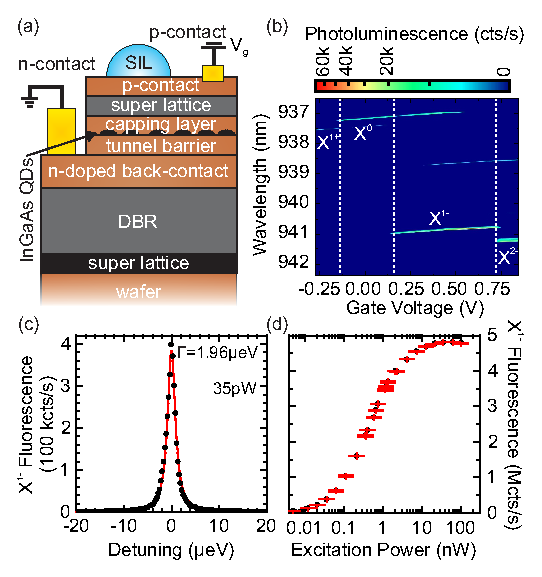
\includegraphics[scale=1]{phonon_paper_suppl_fig1_QD_structure_comp.eps}
	\caption{
	\textbf{Resonance fluorescence spectroscopy on a quantum dot (QD) with narrowband continuous wave excitation.}
	\textbf{(a)} the n-i-p layer structure.
	\textbf{(b)} Non-resonant photoluminescence of the QD as a function of the gate voltage $V_g$.
	\textbf{(c)} Narrowband, resonant excitation performance of the QD. An example spectrum showing the resonance fluorescence signal as function of laser detuning at an excitation power of \SI{35}{\pico\watt}. A Lorentzian fit (red solid line) to the black data points shows a FWHM of \SI{1.96}{\micro\electronvolt}.
	\textbf{(d)} Resonance fluorescence signal with resonant continuous wave excitation as a function of the excitation power.
	}
	\label{fig:sfig1}
\end{figure}


In the experiment the n-contact is grounded and a gate voltage $V_g$ is applied to the p-contact. The gate voltage allows control over the charge: single electrons can be loaded into the QD; furthermore, excitonic resonances can be shifted by the DC Stark effect \cite{Warburton2000,Dalgarno2008,Warburton2013}. Fig.\ \ref{fig:sfig1}(b) shows the photoluminescence from a single QD following non-resonant excitation at \SI{830}{\nano\meter} (excitation into the wetting layer). Several charging plateaus are clearly visible in the photoluminescence. They correspond to optical transitions from an excited state to a ground state with different charge: $\ket{\mathrm{X}^{1+}}\rightarrow\ket{\mathrm{h}^{1+}}$, $\ket{\mathrm{X}^0}\rightarrow\ket{0}$, $\ket{\mathrm{X}^{1-}}\rightarrow\ket{\mathrm{e}^{1-}}$ and $\ket{\mathrm{X}^{2-}}\rightarrow\ket{\mathrm{e}^{2-}}$, with $\ket{\mathrm{h}^{1+}}$ and $\ket{\mathrm{e}^{1-}}$ representing a single hole and single electron, respectively. The DC Stark shift is from red to blue with increasing $V_g$ and can be seen clearly. 
We note that the X$^0$ plateau overlaps with the X$^{1-}$ plateau only with non-resonant excitation. We attribute this overlap to  the occasional decay of the $\ket{\mathrm{X}^{1-}}$ via an Auger process \cite{Kurzmann2016}.

\subsection{Resonance fluorescence with continuous wave excitation}


In resonance fluorescence spectroscopy we investigate the QD characteristics with a narrow band (linewidth in sub \si{\pico\meter} range) excitation laser.
The scattering induced by resonant excitation is detected. Back-reflected laser light is suppressed with a dark-field technique leading to an extinction of $10^7$:1 \cite{Kuhlmann2013_NatPhys,Kuhlmann2013_RSI}. A typical $\mathrm{X}^{1-}$ spectrum from the QD at low excitation power is depicted in Fig.\ \ref{fig:sfig1}(c). The linewidth, measured here slowly, is around \SI{2}{\micro\electronvolt} well below saturation, approximately 2.5 times larger than the transform limit \cite{Kuhlmann2013_NatPhys}. A signal to background ratio of more than 1,000: is achieved with linearly polarized excitation. With increasing excitation power the linewidth broadens (power broadening) and the resonance fluorescence signal increases reaching a saturation count-rate of \SI{5}{\mega cts\per\sec} (\SI{5}{\mega\hertz}), Fig.\ \ref{fig:sfig1}(d). This signal is about 10 times more than from QDs in typical n-i-Schottky samples \cite{Kuhlmann2013_NatPhys}. The signal is measured with a single photon avalanche photodiode (SPAD) with an efficiency of 20\% at these wavelengths. Throughout, the stated count-rates are the bare count rates and are not corrected for instance for the poor SPAD quantum efficiency. The photon extraction efficiency from single QDs in the n-i-p device is around 10\%, a success resulting from several improvements in the sample design as discussed above: the n-i-p type features a DBR and a transparent epitaxial gate.

\begin{table}[t]
	\begin{tabular}{llr}
	\hline \hline
	Function & Material & Thickness \\ \hline
	wafer & GaAs &\\
	buffer & GaAs & \SI{50}{\nano\meter}\\
	superlattice, 18 periods & GaAs, AlAs & \SI{72}{\nano\meter}\\
	DBR, 16 periods & GaAs, AlAs & \SI{2400}{\nano\meter}\\
	spacer & GaAs & \SI{57.3}{\nano\meter}\\
	electron reservoir, back contact & GaAs:Si & \SI{50}{\nano\meter}\\
	tunnel barrier & GaAs & \SI{30}{\nano\meter}\\
	InGaAs QDs & InAs & $\sim$1.6 ML\\
	capping layer & GaAs & \SI{153}{\nano\meter}\\
	blocking barrier, 46 periods & AlAs, GaAs & \SI{184}{\nano\meter}\\
	p-doped top contact & GaAs:C & \SI{30.5}{\nano\meter}\\
	undoped spacer & GaAs & \SI{1}{\nano\meter}\\
	etch stop & AlAs & \SI{2}{\nano\meter}\\
	top capping layer & GaAs & \SI{44}{\nano\meter}\\
		\hline \hline
	\end{tabular}
	\caption{Layers of the n-i-p diode. QDs are formed by depositing 1.6 monolayers (ML) of InAs. The distributed Bragg reflector (DBR) increases the photon extraction efficiency.}
	\label{tab:nip}
\end{table}



\subsection{Resonance fluorescence with pulsed excitation}

\begin{figure}[b]{}
	\centering
	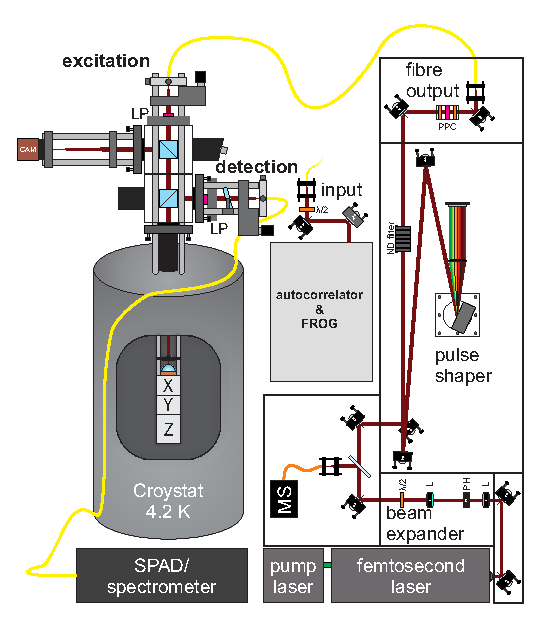
\includegraphics[scale=1]{phonon_paper_suppl_fig2_setup.eps}
	\caption{
	\textbf{Scheme of the complete set-up.} Ultra-short pulses were manipulated in a pulse-shaper, coupled into a single mode glass fiber and sent to a confocal microscope mounted on a bath cryostat. The pulses were characterized with a combination of autocorrelator and frequency-resolved-gating (FROG). The sample is held at a temperature of \SI{4.2}{\kelvin} in the bath croystat on an xyz-positioner. A mini spectrometer (MS) measures the spectral profile of the pulses.
	}
	\label{fig:sfig2}
\end{figure}

With pulsed excitation, we use the full spectrum of \SI{130}{\femto\second} transform-limited ``ultra-fast" pulses, again exciting the QD resonantly. The spectral full-width-at-half-maximum (FWHM) of the pulse is $\Delta \lambda=\SI{10}{\nano\meter}$. With this bandwidth we address the ground state transition for the particular charge state set by the gate voltage (but not higher energy transitions). The resonance fluorescence of the QD is detected with a grating spectrometer.

A scheme of the complete set-up is shown in Fig.\ \ref{fig:sfig2}. The ultra-fast pulses from a mode-locked femtosecond laser are expanded and sent into a compact pulse-shaper. The pulse-shaper retains all the spectral components and controls the amount of chirp as described below. From here the pulses pass through power control and polarization optics and are then coupled into a single mode optical fiber. The fiber transports the pulses to a confocal microscope. In the microscope, the excitation pulses pass through a linear polarizer, two beam-splitters and are sent to the objective at cryogenic temperature (4.2 K). The objective, an aspherical lens with a numerical aperture of 0.68, focuses the light onto the sample. The sample is held on a stack of piezo-steppers which allows a particular QD to be placed within the focal spot of the microscope. This process is aided by the in situ diagnostics provided by a camera image of the focus. Light scattered by the QD is collected and coupled into the detection fiber. The back-reflected laser light is suppressed by a second linear polarizer whose axis is orthogonal to the axis of the polarizer in the excitation stage. The resonance fluorescence signal is detected directly with a SPAD (continuous wave excitation) or with a spectrometer-CCD camera (pulsed excitation).

\begin{figure}[b]{}
	\centering
	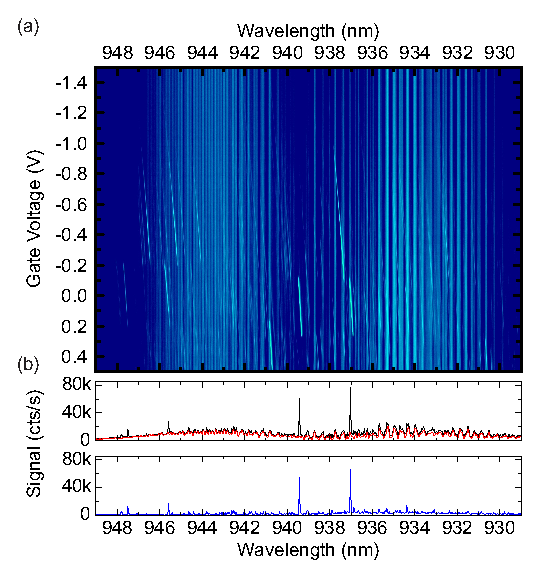
\includegraphics[scale=1]{phonon_paper_suppl_fig3_background_comp.eps}
	\caption{
	\textbf{Laser background subtraction in resonance fluorescence spectroscopy using broadband, pulsed excitation.}
	\textbf{(a)} The resonance fluorescence signal as a function of gate voltage without background subtraction measured with an excitation power of \SI{\sim8}{\micro\watt} corresponding to a pulse area of around 3 $\pi$.
	\textbf{(b)} One spectrum from (a) at a gate voltage of \SI{-0.012}{\volt} is shown as the black curve in the upper panel. Distinct peaks from the exciton and trion are visible toegther with a broad laser background. The reconstructed laser background (from all spectra in (a)) is shown in red. The blue curve in the lower panel shows the difference between the black and the red curve, the resulting signal after background subtraction.
	}
	\label{fig:sfig3}
\end{figure}

Detecting resonance fluorescence with pulsed excitation also depends on suppressing the reflected laser light with the polarization-based dark-field technique. However, owing to the wavelength dependence of the polarization optics, the laser suppression of a broadband pulsed laser is less effective than with the narrowband continuous wave laser: we reach an extinction ratio of typically $10^5$:1 with broadband excitation. We use in addition the spectral mismatch between the broadband laser and the narrowband resonance fluorescence to increase the extinction ratio, Fig.\ \ref{fig:sfig3}. The laser background falling on the CCD camera does not depend on the gate voltage, Fig.\ \ref{fig:sfig3}(a), such that we can use the gate voltage dependence of the QD emission to construct the laser background spectrum. The resulting residual laser background is shown in Fig.\ \ref{fig:sfig3}(b) in red. The spectral shape is explained by the Gaussian spectral shape of the excitation laser along with the quadratic function of laser suppression: the laser suppression is most effective at its alignment wavelength and then decays quadratically in wavelength superimposed by interference fringes. A typical spectrum measured at $V_g=\SI{-12}{\milli\volt}$ is shown in black. Sharp emission peaks from the exciton and biexciton appear on top of the laser background. The signal after background subtraction is shown in the lower plot in blue. Before background subtraction, the maximum signal to background ratio in a narrow spectral window around the emission line is 22:1.

The measurement of emission linewidths in resonance fluorescence with broadband excitation is limited by the resolution of the spectrometer. Hence, we can only state that these linewidths are below \SI{30}{\micro\electronvolt}, as depicted in the spectrum in Fig.\ 1 of the main paper.


\subsection{Pulse shaping: introducing chirp}\label{sec:pulseshaper}
Chirp is introduced into the transform-limited laser pulses by a compact, folded $4f$ pulse-shaper \cite{Martinez1987,Weiner1992}. The scheme is depicted in Fig.\ 1 of the main paper. The unchirped pulse is diffracted by a high resolution, blazed grating (1,800 grooves per mm) and then focused by a lens onto a mirror positioned in the focal plane. From here the light travels back under a small angle with respect to the diffraction plane allowing a spatial separation of incoming and outgoing pulses. The distance between grating and lens controls the chirp \cite{Martinez1987}. The lens and the mirror are mounted on a translation platform. Moving the platform with respect to the grating changes the chirp: if the distance matches the focal length of the lens the chirp is zero, a larger (smaller) distance leads to negative (positive) chirp. The temporal duration of the pulses exiting the laser is \SI{130}{\femto\second} (intensity FWHM); the temporal duration can be stretched up to \SI{15}{\pico\second} corresponding to a chirp in the range from \SI{-0.7}{\pico\second\squared} to \SI{+0.7}{\pico\second\squared}. 

We characterized the chirp with a combination of a FROG and autocorrelator. This allows us to reveal the presence of any high-order phase terms and prevent them by an optimal adjustment of the pulse-shaper. The chirp is measured both in the free space mode and also after the optical single mode fiber in order to determine the sign of the chirp and to compensate for the chirp introduced by the fiber itself.

\section{Theoretical Model}
For the theoretical calculations we use the standard model of a two-level system coupled to longitudinal phonons. For clarity, we outline here the details of the model.

\subsection{Hamiltonian}
We can divide the Hamiltonian $H$ of the system into four parts with
\begin{align*}
H = H_{\textrm{c}} + H_{\textrm{c-l}} + H_{\textrm{ph}} + H_{\textrm{c-ph}},
\end{align*}
where $H_{\textrm{c}}$ denotes the electronic structure, $H_{\textrm{c-l}}$ describes the carrier-light coupling and $H_{\textrm{ph}}+H_{\textrm{c-ph}} $ the phonon part. 

For the electronic structure we take a two-level system, which consists of the ground state $\ket{\mathrm{e}^{1-}}$ and the single exciton state $\ket{\mathrm{X}^{1-}}$ with the Hamiltonian
\begin{align*}
H_{\textrm{c}} = \hbar\omega_{\mathrm{X}^{1-}}\ket{\mathrm{X}^{1-}}\bra{\mathrm{X}^{1-}},
\end{align*}
where $\hbar\omega_{\mathrm{X}^{1-}}$ denotes the energy of the negative trion. The energy of the ground state has been set to zero.

The carrier-light interaction is modeled in the usual dipole and rotating wave approximation. For this two-level system we have
\begin{equation*}
H_{\textrm{c-l}} = \, \frac{\hbar}{2}\left(\Omega(t)|\mathrm{X}^{1-}\rangle\langle \mathrm{e}^{1-}| + \Omega^*(t)|\mathrm{e}^{1-}\rangle\langle \mathrm{X}^{1-}|\right). \\
\end{equation*}
where $\hbar\Omega(t)=2\mathbf{M}\cdot \mathbf{E}(t)$, with $\mathbf{E}(t)$ the positive frequency component of the electric field of the laser pulse; $\mathbf{M}$ denotes the dipole matrix element. 

The main source of decoherence in QDs is caused by the coupling to longitudinal acoustic (LA) phonons which are treated as bulk-like due to the small acoustic mismatch between the QD area and the surrounding material \cite{Reiter2014}. The Hamiltonian of the free phonons reads
\begin{align*}
H_{\textrm{ph}} = \hbar\sum_{\mathbf{q}}\omega_{\mathbf{q}}b^\dag_{\mathbf{q}}b_{\mathbf{q}},
\end{align*}
where $b^\dag_{\mathbf{q}}$ ($b_{\mathbf{q}}$) is the creation (annihilation) operator of a phonon with wave vector $\mathbf{q}$ and frequency $\omega_{\mathbf{q}} = c_{s}|\mathbf{q}|$, $c_{s}$ being the sound velocity.

The carrier-phonon interaction is modeled by a pure-dephasing Hamiltonian using the deformation potential coupling mechanism. The corresponding Hamiltonian is given by
\begin{align*}
H_{\textrm{c-ph}} = \hbar\sum_{\mathbf{q}} \left(g_{\mathbf{q}}b_{\mathbf{q}} + g^*_{\mathbf{q}}b^\dag_{\mathbf{q}}\right) |\mathrm{X}^{1-} \rangle\langle \mathrm{X}^{1-}| .
\end{align*}
The main coupling mechanism is the deformation potential coupling with the coupling matrix element for the electrons and holes
\[
	g_{\mathbf{q}}^{e/h}=\sqrt{\frac{q}{2V\rho\hbar c_{s}}}D_{e/h}F_{\mathbf{q}}^{e/h},
\]
where $V$ is the normalization volume, $\rho$ the mass density of the crystal, and $D_{e/h}$ the deformation potential coupling constant for electrons/holes. As parameters we take the standard GaAs parameter listed in Tab.~\ref{tab:para}. The exciton coupling matrix element is obtained by $g_{\mathbf{q}} = g_{\mathbf{q}}^{e}- g_{\mathbf{q}}^{h}$.

The form factor $F_{\mathbf{q}}^{e/h}$ accounts for the bound states of the QD and, thus, for the geometry of the QD. We assume a harmonic confinement potential in a lens-shaped QD yielding the form factor
\[
	F_{\mathbf{q}}^{e/h}=\exp\left[-\frac{1}{4}\left(q_z^2 a_{e/h,z}^2+q_{r}^2a_{e/h,r}^2\right)\right].
\]
$q_z$ is the wave vector in the $z$-direction; $q_{r}$ is the in-plane wave vector. $a_{e/h,z}$ and $a_{e/h,r}$ are the electron/hole localization lengths in the $z$-direction and in the $(x,y)$-plane direction, respectively. We used $a_{e,z}=1.5$~nm and $a_{e,z}= 5.7$~nm, thereby modelling a flat QD. The ratio between electron and hole localization lengths is taken to be $a_h/a_e=0.77$ for both directions \cite{warburton2002gia}.

\begin{table}[t]
\begin{tabular}{llr}
\hline \hline
Parameter & & Value \\ \hline
density & $\rho$& $5370\,$kg/m$^3$\\
sound velocity & $c_{s}$ & $5.1\,$nm/ps\\
electron deformation potential constant &$D_e$&$7$~eV\\
hole deformation potential constant &$D_h$&	$-3.5$~eV\\
	\hline \hline
\end{tabular}
\caption{\label{tab:para} Material parameters used in the calculation.}
\end{table}

Before the laser pulse, we assume that the electronic system is in the
ground state and the phonon system is in a thermal equilibrium given by
a Bose distribution at temperature $T$ with $\langle
b^\dag_{\mathbf{q}}b_{\mathbf{q}} \rangle = n_q(T) = 1/(e^{\hbar c_s
q/k_B T}+1)$  with $k_B$ the Boltzmann constant. If not denoted
otherwise, we use liquid helium temperature at $T=4~K$. Assuming an
initially uncorrelated state, we can take the product state between
carrier and phonon system as initial condition for the dynamics.

Using this Hamiltonian we set up the equations of motion in the density matrix formalism which leads to an infinite hierarchy of phonon-assisted variables. We truncate this hierarchy using a fourth-order correlation expansion, which yields reliable results for the carrier-dynamics in a QD \cite{Reiter2014,Luker2012,glassl2011lon}. The equations of motion of the two-level model can be found, e.g., in Ref.~\cite{krugel2006bac}. 


% Create the reference section using BibTeX:
%\bibliography{phonon_paper_bib_06}
% Run this once to generate your BBL file. Then copy the contents of your BBL file into your main latex file, commenting out "\bibliography"

\begin{thebibliography}{14}%
\makeatletter
\providecommand \@ifxundefined [1]{%
 \@ifx{#1\undefined}
}%
\providecommand \@ifnum [1]{%
 \ifnum #1\expandafter \@firstoftwo
 \else \expandafter \@secondoftwo
 \fi
}%
\providecommand \@ifx [1]{%
 \ifx #1\expandafter \@firstoftwo
 \else \expandafter \@secondoftwo
 \fi
}%
\providecommand \natexlab [1]{#1}%
\providecommand \enquote  [1]{``#1''}%
\providecommand \bibnamefont  [1]{#1}%
\providecommand \bibfnamefont [1]{#1}%
\providecommand \citenamefont [1]{#1}%
\providecommand \href@noop [0]{\@secondoftwo}%
\providecommand \href [0]{\begingroup \@sanitize@url \@href}%
\providecommand \@href[1]{\@@startlink{#1}\@@href}%
\providecommand \@@href[1]{\endgroup#1\@@endlink}%
\providecommand \@sanitize@url [0]{\catcode `\\12\catcode `\$12\catcode
  `\&12\catcode `\#12\catcode `\^12\catcode `\_12\catcode `\%12\relax}%
\providecommand \@@startlink[1]{}%
\providecommand \@@endlink[0]{}%
\providecommand \url  [0]{\begingroup\@sanitize@url \@url }%
\providecommand \@url [1]{\endgroup\@href {#1}{\urlprefix }}%
\providecommand \urlprefix  [0]{URL }%
\providecommand \Eprint [0]{\href }%
\providecommand \doibase [0]{http://dx.doi.org/}%
\providecommand \selectlanguage [0]{\@gobble}%
\providecommand \bibinfo  [0]{\@secondoftwo}%
\providecommand \bibfield  [0]{\@secondoftwo}%
\providecommand \translation [1]{[#1]}%
\providecommand \BibitemOpen [0]{}%
\providecommand \bibitemStop [0]{}%
\providecommand \bibitemNoStop [0]{.\EOS\space}%
\providecommand \EOS [0]{\spacefactor3000\relax}%
\providecommand \BibitemShut  [1]{\csname bibitem#1\endcsname}%
\let\auto@bib@innerbib\@empty
%</preamble>
\bibitem [{\citenamefont {Prechtel}\ \emph {et~al.}(2016)\citenamefont
  {Prechtel}, \citenamefont {Kuhlmann}, \citenamefont {Houel}, \citenamefont
  {Ludwig}, \citenamefont {Valentin}, \citenamefont {Wieck},\ and\
  \citenamefont {Warburton}}]{Prechtel2016}%
  \BibitemOpen
  \bibfield  {author} {\bibinfo {author} {\bibfnamefont {J.~H.}\ \bibnamefont
  {Prechtel}}, \bibinfo {author} {\bibfnamefont {A.~V.}\ \bibnamefont
  {Kuhlmann}}, \bibinfo {author} {\bibfnamefont {J.}~\bibnamefont {Houel}},
  \bibinfo {author} {\bibfnamefont {A.}~\bibnamefont {Ludwig}}, \bibinfo
  {author} {\bibfnamefont {S.~R.}\ \bibnamefont {Valentin}}, \bibinfo {author}
  {\bibfnamefont {A.~D.}\ \bibnamefont {Wieck}}, \ and\ \bibinfo {author}
  {\bibfnamefont {R.~J.}\ \bibnamefont {Warburton}},\ }\href {\doibase
  10.1038/nmat4704} {\bibfield  {journal} {\bibinfo  {journal} {Nat. Mater.}\
  }\textbf {\bibinfo {volume} {15}},\ \bibinfo {pages} {981} (\bibinfo {year}
  {2016})}\BibitemShut {NoStop}%
\bibitem [{\citenamefont {Warburton}\ \emph {et~al.}(2000)\citenamefont
  {Warburton}, \citenamefont {Schäflein}, \citenamefont {Haft}, \citenamefont
  {Bickel}, \citenamefont {Lorke}, \citenamefont {Karrai}, \citenamefont
  {Garcia}, \citenamefont {Schoenfeld},\ and\ \citenamefont
  {Petroff}}]{Warburton2000}%
  \BibitemOpen
  \bibfield  {author} {\bibinfo {author} {\bibfnamefont {R.~J.}\ \bibnamefont
  {Warburton}}, \bibinfo {author} {\bibfnamefont {C.}~\bibnamefont
  {Schäflein}}, \bibinfo {author} {\bibfnamefont {D.}~\bibnamefont {Haft}},
  \bibinfo {author} {\bibfnamefont {F.}~\bibnamefont {Bickel}}, \bibinfo
  {author} {\bibfnamefont {A.}~\bibnamefont {Lorke}}, \bibinfo {author}
  {\bibfnamefont {K.}~\bibnamefont {Karrai}}, \bibinfo {author} {\bibfnamefont
  {J.~M.}\ \bibnamefont {Garcia}}, \bibinfo {author} {\bibfnamefont
  {W.}~\bibnamefont {Schoenfeld}}, \ and\ \bibinfo {author} {\bibfnamefont
  {P.~M.}\ \bibnamefont {Petroff}},\ }\href {\doibase 10.1038/35016030}
  {\bibfield  {journal} {\bibinfo  {journal} {Nature}\ }\textbf {\bibinfo
  {volume} {405}},\ \bibinfo {pages} {926} (\bibinfo {year}
  {2000})}\BibitemShut {NoStop}%
\bibitem [{\citenamefont {Dalgarno}\ \emph {et~al.}(2008)\citenamefont
  {Dalgarno}, \citenamefont {Smith}, \citenamefont {McFarlane}, \citenamefont
  {Gerardot}, \citenamefont {Karrai}, \citenamefont {Badolato}, \citenamefont
  {Petroff},\ and\ \citenamefont {Warburton}}]{Dalgarno2008}%
  \BibitemOpen
  \bibfield  {author} {\bibinfo {author} {\bibfnamefont {P.~A.}\ \bibnamefont
  {Dalgarno}}, \bibinfo {author} {\bibfnamefont {J.~M.}\ \bibnamefont {Smith}},
  \bibinfo {author} {\bibfnamefont {J.}~\bibnamefont {McFarlane}}, \bibinfo
  {author} {\bibfnamefont {B.~D.}\ \bibnamefont {Gerardot}}, \bibinfo {author}
  {\bibfnamefont {K.}~\bibnamefont {Karrai}}, \bibinfo {author} {\bibfnamefont
  {A.}~\bibnamefont {Badolato}}, \bibinfo {author} {\bibfnamefont {P.~M.}\
  \bibnamefont {Petroff}}, \ and\ \bibinfo {author} {\bibfnamefont {R.~J.}\
  \bibnamefont {Warburton}},\ }\href {\doibase 10.1103/PhysRevB.77.245311}
  {\bibfield  {journal} {\bibinfo  {journal} {Phys. Rev. B}\ }\textbf {\bibinfo
  {volume} {77}},\ \bibinfo {pages} {245311} (\bibinfo {year}
  {2008})}\BibitemShut {NoStop}%
\bibitem [{\citenamefont {Warburton}(2013)}]{Warburton2013}%
  \BibitemOpen
  \bibfield  {author} {\bibinfo {author} {\bibfnamefont {R.~J.}\ \bibnamefont
  {Warburton}},\ }\href {\doibase 10.1038/nmat3585} {\bibfield  {journal}
  {\bibinfo  {journal} {Nat. Mater.}\ }\textbf {\bibinfo {volume} {12}},\
  \bibinfo {pages} {483} (\bibinfo {year} {2013})}\BibitemShut {NoStop}%
\bibitem [{\citenamefont {Kurzmann}\ \emph {et~al.}(2016)\citenamefont
  {Kurzmann}, \citenamefont {Ludwig}, \citenamefont {Wieck}, \citenamefont
  {Lorke},\ and\ \citenamefont {Geller}}]{Kurzmann2016}%
  \BibitemOpen
  \bibfield  {author} {\bibinfo {author} {\bibfnamefont {A.}~\bibnamefont
  {Kurzmann}}, \bibinfo {author} {\bibfnamefont {A.}~\bibnamefont {Ludwig}},
  \bibinfo {author} {\bibfnamefont {A.~D.}\ \bibnamefont {Wieck}}, \bibinfo
  {author} {\bibfnamefont {A.}~\bibnamefont {Lorke}}, \ and\ \bibinfo {author}
  {\bibfnamefont {M.}~\bibnamefont {Geller}},\ }\href {\doibase
  10.1021/acs.nanolett.6b01082} {\bibfield  {journal} {\bibinfo  {journal}
  {Nano Lett.}\ }\textbf {\bibinfo {volume} {16}},\ \bibinfo {pages} {3367}
  (\bibinfo {year} {2016})}\BibitemShut {NoStop}%
\bibitem [{\citenamefont {Kuhlmann}\ \emph
  {et~al.}(2013{\natexlab{a}})\citenamefont {Kuhlmann}, \citenamefont {Houel},
  \citenamefont {Ludwig}, \citenamefont {Greuter}, \citenamefont {Reuter},
  \citenamefont {Wieck}, \citenamefont {Poggio},\ and\ \citenamefont
  {Warburton}}]{Kuhlmann2013_NatPhys}%
  \BibitemOpen
  \bibfield  {author} {\bibinfo {author} {\bibfnamefont {A.~V.}\ \bibnamefont
  {Kuhlmann}}, \bibinfo {author} {\bibfnamefont {J.}~\bibnamefont {Houel}},
  \bibinfo {author} {\bibfnamefont {A.}~\bibnamefont {Ludwig}}, \bibinfo
  {author} {\bibfnamefont {L.}~\bibnamefont {Greuter}}, \bibinfo {author}
  {\bibfnamefont {D.}~\bibnamefont {Reuter}}, \bibinfo {author} {\bibfnamefont
  {A.~D.}\ \bibnamefont {Wieck}}, \bibinfo {author} {\bibfnamefont
  {M.}~\bibnamefont {Poggio}}, \ and\ \bibinfo {author} {\bibfnamefont {R.~J.}\
  \bibnamefont {Warburton}},\ }\href {\doibase 10.1038/nphys2688} {\bibfield
  {journal} {\bibinfo  {journal} {Nat. Phys.}\ }\textbf {\bibinfo {volume}
  {9}},\ \bibinfo {pages} {570} (\bibinfo {year}
  {2013}{\natexlab{a}})}\BibitemShut {NoStop}%
\bibitem [{\citenamefont {Kuhlmann}\ \emph
  {et~al.}(2013{\natexlab{b}})\citenamefont {Kuhlmann}, \citenamefont {Houel},
  \citenamefont {Brunner}, \citenamefont {Ludwig}, \citenamefont {Reuter},
  \citenamefont {Wieck},\ and\ \citenamefont {Warburton}}]{Kuhlmann2013_RSI}%
  \BibitemOpen
  \bibfield  {author} {\bibinfo {author} {\bibfnamefont {A.~V.}\ \bibnamefont
  {Kuhlmann}}, \bibinfo {author} {\bibfnamefont {J.}~\bibnamefont {Houel}},
  \bibinfo {author} {\bibfnamefont {D.}~\bibnamefont {Brunner}}, \bibinfo
  {author} {\bibfnamefont {A.}~\bibnamefont {Ludwig}}, \bibinfo {author}
  {\bibfnamefont {D.}~\bibnamefont {Reuter}}, \bibinfo {author} {\bibfnamefont
  {A.~D.}\ \bibnamefont {Wieck}}, \ and\ \bibinfo {author} {\bibfnamefont
  {R.~J.}\ \bibnamefont {Warburton}},\ }\href {\doibase 10.1063/1.4813879}
  {\bibfield  {journal} {\bibinfo  {journal} {Rev. Sci. Instrum.}\ }\textbf
  {\bibinfo {volume} {84}},\ \bibinfo {pages} {073905} (\bibinfo {year}
  {2013}{\natexlab{b}})}\BibitemShut {NoStop}%
\bibitem [{\citenamefont {Martinez}(1987)}]{Martinez1987}%
  \BibitemOpen
  \bibfield  {author} {\bibinfo {author} {\bibfnamefont {O.}~\bibnamefont
  {Martinez}},\ }\href {\doibase 10.1109/JQE.1987.1073201} {\bibfield
  {journal} {\bibinfo  {journal} {IEEE J. Quantum Electron.}\ }\textbf
  {\bibinfo {volume} {23}},\ \bibinfo {pages} {59} (\bibinfo {year}
  {1987})}\BibitemShut {NoStop}%
\bibitem [{\citenamefont {Weiner}\ \emph {et~al.}(1992)\citenamefont {Weiner},
  \citenamefont {Leaird}, \citenamefont {Patel},\ and\ \citenamefont
  {Wullert}}]{Weiner1992}%
  \BibitemOpen
  \bibfield  {author} {\bibinfo {author} {\bibfnamefont {A.~M.}\ \bibnamefont
  {Weiner}}, \bibinfo {author} {\bibfnamefont {D.~E.}\ \bibnamefont {Leaird}},
  \bibinfo {author} {\bibfnamefont {J.~S.}\ \bibnamefont {Patel}}, \ and\
  \bibinfo {author} {\bibfnamefont {J.~R.}\ \bibnamefont {Wullert}},\ }\href
  {\doibase 10.1109/3.135209} {\bibfield  {journal} {\bibinfo  {journal} {IEEE
  J. Quantum Electron.}\ }\textbf {\bibinfo {volume} {28}},\ \bibinfo {pages}
  {908} (\bibinfo {year} {1992})}\BibitemShut {NoStop}%
\bibitem [{\citenamefont {Reiter}\ \emph {et~al.}(2014)\citenamefont {Reiter},
  \citenamefont {Kuhn}, \citenamefont {Gl{\"{a}}ssl},\ and\ \citenamefont
  {Axt}}]{Reiter2014}%
  \BibitemOpen
  \bibfield  {author} {\bibinfo {author} {\bibfnamefont {D.~E.}\ \bibnamefont
  {Reiter}}, \bibinfo {author} {\bibfnamefont {T.}~\bibnamefont {Kuhn}},
  \bibinfo {author} {\bibfnamefont {M.}~\bibnamefont {Gl{\"{a}}ssl}}, \ and\
  \bibinfo {author} {\bibfnamefont {V.~M.}\ \bibnamefont {Axt}},\ }\href
  {\doibase 10.1088/0953-8984/26/42/423203} {\bibfield  {journal} {\bibinfo
  {journal} {J. Phys. Condens. Matter}\ }\textbf {\bibinfo {volume} {26}},\
  \bibinfo {pages} {423203} (\bibinfo {year} {2014})}\BibitemShut {NoStop}%
\bibitem [{\citenamefont {Warburton}\ \emph {et~al.}(2002)\citenamefont
  {Warburton}, \citenamefont {Schulhauser}, \citenamefont {Haft}, \citenamefont
  {Sch{\"a}flein}, \citenamefont {Karrai}, \citenamefont {Garcia},
  \citenamefont {Schoenfeld},\ and\ \citenamefont
  {Petroff}}]{warburton2002gia}%
  \BibitemOpen
  \bibfield  {author} {\bibinfo {author} {\bibfnamefont {R.~J.}\ \bibnamefont
  {Warburton}}, \bibinfo {author} {\bibfnamefont {C.}~\bibnamefont
  {Schulhauser}}, \bibinfo {author} {\bibfnamefont {D.}~\bibnamefont {Haft}},
  \bibinfo {author} {\bibfnamefont {C.}~\bibnamefont {Sch{\"a}flein}}, \bibinfo
  {author} {\bibfnamefont {K.}~\bibnamefont {Karrai}}, \bibinfo {author}
  {\bibfnamefont {J.~M.}\ \bibnamefont {Garcia}}, \bibinfo {author}
  {\bibfnamefont {W.}~\bibnamefont {Schoenfeld}}, \ and\ \bibinfo {author}
  {\bibfnamefont {P.~M.}\ \bibnamefont {Petroff}},\ }\href@noop {} {\bibfield
  {journal} {\bibinfo  {journal} {Phys. Rev. B}\ }\textbf {\bibinfo {volume}
  {65}},\ \bibinfo {pages} {113303} (\bibinfo {year} {2002})}\BibitemShut
  {NoStop}%
\bibitem [{\citenamefont {L{\"{u}}ker}\ \emph {et~al.}(2012)\citenamefont
  {L{\"{u}}ker}, \citenamefont {Gawarecki}, \citenamefont {Reiter},
  \citenamefont {Grodecka-Grad}, \citenamefont {Axt}, \citenamefont
  {Machnikowski},\ and\ \citenamefont {Kuhn}}]{Luker2012}%
  \BibitemOpen
  \bibfield  {author} {\bibinfo {author} {\bibfnamefont {S.}~\bibnamefont
  {L{\"{u}}ker}}, \bibinfo {author} {\bibfnamefont {K.}~\bibnamefont
  {Gawarecki}}, \bibinfo {author} {\bibfnamefont {D.~E.}\ \bibnamefont
  {Reiter}}, \bibinfo {author} {\bibfnamefont {A.}~\bibnamefont
  {Grodecka-Grad}}, \bibinfo {author} {\bibfnamefont {V.~M.}\ \bibnamefont
  {Axt}}, \bibinfo {author} {\bibfnamefont {P.}~\bibnamefont {Machnikowski}}, \
  and\ \bibinfo {author} {\bibfnamefont {T.}~\bibnamefont {Kuhn}},\ }\href
  {\doibase 10.1103/PhysRevB.85.121302} {\bibfield  {journal} {\bibinfo
  {journal} {Phys. Rev. B}\ }\textbf {\bibinfo {volume} {85}},\ \bibinfo
  {pages} {121302} (\bibinfo {year} {2012})}\BibitemShut {NoStop}%
\bibitem [{\citenamefont {Gl\"assl}\ \emph {et~al.}(2011)\citenamefont
  {Gl\"assl}, \citenamefont {Vagov}, \citenamefont {L\"uker}, \citenamefont
  {Reiter}, \citenamefont {Croitoru}, \citenamefont {Machnikowski},
  \citenamefont {Axt},\ and\ \citenamefont {Kuhn}}]{glassl2011lon}%
  \BibitemOpen
  \bibfield  {author} {\bibinfo {author} {\bibfnamefont {M.}~\bibnamefont
  {Gl\"assl}}, \bibinfo {author} {\bibfnamefont {A.}~\bibnamefont {Vagov}},
  \bibinfo {author} {\bibfnamefont {S.}~\bibnamefont {L\"uker}}, \bibinfo
  {author} {\bibfnamefont {D.~E.}\ \bibnamefont {Reiter}}, \bibinfo {author}
  {\bibfnamefont {M.~D.}\ \bibnamefont {Croitoru}}, \bibinfo {author}
  {\bibfnamefont {P.}~\bibnamefont {Machnikowski}}, \bibinfo {author}
  {\bibfnamefont {V.~M.}\ \bibnamefont {Axt}}, \ and\ \bibinfo {author}
  {\bibfnamefont {T.}~\bibnamefont {Kuhn}},\ }\href {\doibase
  10.1103/PhysRevB.84.195311} {\bibfield  {journal} {\bibinfo  {journal} {Phys.
  Rev. B}\ }\textbf {\bibinfo {volume} {84}},\ \bibinfo {pages} {195311}
  (\bibinfo {year} {2011})}\BibitemShut {NoStop}%
\bibitem [{\citenamefont {Kr{\"{u}}gel}\ \emph {et~al.}(2006)\citenamefont
  {Kr{\"{u}}gel}, \citenamefont {Axt},\ and\ \citenamefont
  {Kuhn}}]{krugel2006bac}%
  \BibitemOpen
  \bibfield  {author} {\bibinfo {author} {\bibfnamefont {A.}~\bibnamefont
  {Kr{\"{u}}gel}}, \bibinfo {author} {\bibfnamefont {V.~M.}\ \bibnamefont
  {Axt}}, \ and\ \bibinfo {author} {\bibfnamefont {T.}~\bibnamefont {Kuhn}},\
  }\href {\doibase 10.1103/PhysRevB.73.035302} {\bibfield  {journal} {\bibinfo
  {journal} {Phys. Rev. B}\ }\textbf {\bibinfo {volume} {73}},\ \bibinfo
  {pages} {035302} (\bibinfo {year} {2006})}\BibitemShut {NoStop}%
\end{thebibliography}%


\end{document}
